\documentclass{beamer}
\usepackage[utf8]{inputenc}
\usepackage[spanish]{babel}
\usepackage{graphicx,hyperref,ru,url}

% The title of the presentation:
%  - first a short version which is visible at the bottom of each slide;
%  - second the full title shown on the title slide;
\title[Inmune competition and cancer dynamics]{
  A mathematical model of inmune competition related to cancer dynamics}

% Optional: a subtitle to be dispalyed on the title slide
\subtitle{By Ilaria Brazzoli, Elena De Angelis and Pierre-Emmanuel Jabin}

% The author(s) of the presentation:
%  - again first a short version to be displayed at the bottom;
%  - next the full list of authors, which may include contact information;
\author[Bartolomé Ortiz Viso]{
  Bartolomé Ortiz Viso \\\medskip
  {\small \url{bortiz@correo.ugr.es}} \\ 
  {\small \url{@bortizmath}}}

% The institute:
%  - to start the name of the university as displayed on the top of each slide
%    this can be adjusted such that you can also create a Dutch version
%  - next the institute information as displayed on the title slide
\institute[Universidad de Granada]{
  EDP de transporte  \\
  Máster en Física y Matemáticas}

% Add a date and possibly the name of the event to the slides
%  - again first a short version to be shown at the bottom of each slide
%  - second the full date and event name for the title slide
\date[17 Enero, 2018]{
  17 Enero, 2018}

\begin{document}

\begin{frame}
  \titlepage
\end{frame}

\begin{frame}
  \frametitle{Índice}

  \tableofcontents
\end{frame}

% Section titles are shown in at the top of the slides with the current section 
% highlighted. Note that the number of sections determines the size of the top 
% bar, and hence the university name and logo. If you do not add any sections 
% they will not be visible.
\section{Introducción}

\begin{frame}
  \frametitle{Introducción}
El desarrollo de la \textbf{teoría cinética de partículas} activas ha supuesto un gran avance para el descubrimiento de nuevos modelos matemáticos en el ámbito de la biología.


\end{frame}

\begin{frame}
	  \begin{columns}[t]
	  
	  	
	  	\column{0.5\textwidth}
	  	La\textbf{ teoría cinética de partículas activas}
	  	$$\downarrow$$
	  	  Marco de desarrollo de \textbf{modelos de competición inmune}.
	  	$$\downarrow$$
	  	\begin{itemize}
	  		\item Podemos pasar de descripciones locales a globales.
	  		\item Introducimos actividades o cualidades celulares.
	  	\end{itemize}
	  		\column{0.5\textwidth}
	  		\begin{figure}[Celulas endoteliales]
	  			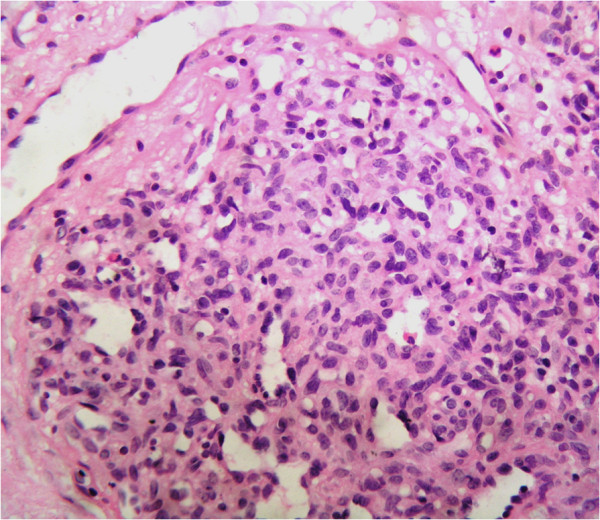
\includegraphics[scale=1]{intro.png}
	  			\caption{Tejido endotelial implicado en competiciones inmunes}
	  			\label{tejido}
	  		\end{figure}
\end{columns}
\end{frame}


\section{Descripción del modelo}

\begin{frame}
  \frametitle{Descripción del modelo}
  \begin{block}{Inmunovigilancia}
    Periodo en el cual el sistema inmune debe reconocer células tumorales durmientes y frenar su avance o erradicarlas.
  \end{block}
 \begin{block}{Poblaciones afectadas}
 	\begin{itemize}
 		\item células endoteliales.
 		\item células del sistema inmune.
 		\item celulas tumorales.
 	\end{itemize}
 \end{block}
\end{frame}

\begin{frame}
	\frametitle{Descripción del modelo}
	\begin{block}{Función de distribución de una partícula generalizada}
		Para cada poblacion en $t\in[0,T]$ definimos:
		$$f_i=f_i(t,u)$$
	\end{block}

	$$
	n_i(t)= n_i [f_i] (t) =\int_{0}^{+\infty} f_i (t, u) du,
	$$	Densidad total o tamaño de población 
	
	$$A_i (t) = A_i [f_i] (t) =\int_{0}^{+\infty}uf_i(t,u),$$
	
	Actividad de cada población.
\end{frame}


\begin{frame}
	\frametitle{Descripción del modelo}
	\begin{enumerate}
		\item La \textbf{proliferación} de las células endoteliales ($A_1$) se ve \textbf{afectada negativamente} por las células tumorales. A su vez, se ve \textbf{afectada positivamente} por la propia reproducción celular.
		\item Las células inmunes tienden a ($A_2$) \textbf{estado centinela} asociado a una constante. Además la actividad tumoral \textbf{provoca} la actividad inmunológica.
		\item Las células tumorales\textbf{ proliferan} y las células inmunes \textbf{destruyen} las células tumorales.
	\end{enumerate}
\end{frame}

\begin{frame}
	\frametitle{Descripción del modelo}
\begin{equation}
\frac{d}{dt}A_1=-A_1(t)A_3(t)+\alpha(A_1)A_1(t),
\end{equation}
\begin{equation}
\frac{d}{dt}A_2=A_2^*-A_2(t)+A_3(t),
\end{equation}
\begin{equation}
\partial_tf_3+\partial_uf_3=r(u)f_3(t,u)-A_2(t)f_3(t,u).
\end{equation}
\end{frame}




\section{Resultados teóricos}

\begin{frame}
	\frametitle{Resultados teóricos}
	\begin{block}{Hipótesis}
		
		\begin{enumerate}[(i)]
			\item $\alpha \in L^\infty[0,+\infty)$, con $A_1^*>0$
			\item $r(u)\in L^\infty[0,+\infty)$ y $r(0)=0$
			\item $r(u)=R^*-(A/u)+O(1/u^2)$ cuando $u\rightarrow\infty$
		\end{enumerate}
		
	\end{block}
	
\end{frame}


\begin{frame}
  \frametitle{Resultados teóricos}
\begin{theorem}
		Suponiendo: $$f_3^0(u)\geq0 \text{ y } \int_{0}^{+\infty}(1+u)f_3^0(u)du<\infty$$
		Entonces existe al menos una solución $(A_1,A_2,A_3)$ para el problema de valores iniciales $(1)-(5)$ en el sentido de las distribuciones, tal que $(A_1,A_2)\in C([0,\infty))$ y $f_3\in L^1((1+u)du)$.
\end{theorem}


\end{frame}



\begin{frame}
	\frametitle{Resultados teóricos}
	\begin{theorem}
	Suponiendo que la condición inicial cumple la condición \ref{cond}, entonces cuando $t\rightarrow\infty$ se tiene:
	\begin{enumerate}
		\item $A_1(t)\rightarrow0$;
		\item $n_3(t)\rightarrow0$;
		\item $A_2(t)\rightarrow R^*$ y $A_3(t)\rightarrow R^*-A_2^*$;
		\item $\exists L(u)\in L^1(du,\mathbb{R})$ y $\exists\phi(t)$de manera que $f_3$ con la adecuada normalización converge a $L(u)$
		$$\int_{\infty}^{\infty}f_3(t,u+t)\frac{e^{Alog(u+t)}}{\phi(t)}-L(u)du\leq\frac{c}{t}$$
		donde $c$ es constante y $A$ es la definida en la hipótesis.
	\end{enumerate}\label{teorema3}
	\end{theorem}
	
	
\end{frame}

\section{Simulaciones numéricas}

\begin{frame}
	\frametitle{Simulaciones numéricas $A_1 = 0.5, A_2 = 0.2, \beta = 1$}
	\begin{figure}
		\centering
		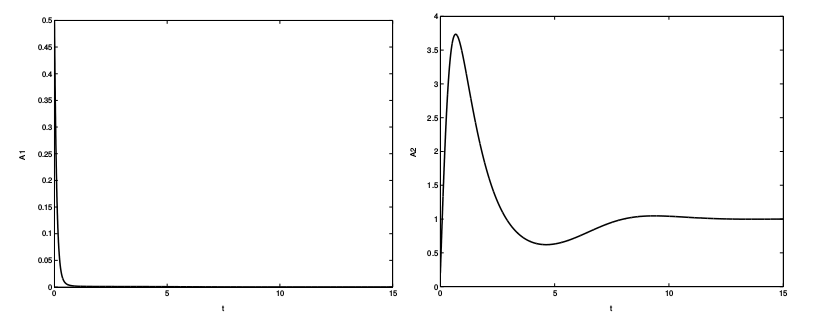
\includegraphics[width=1\textwidth]{test2A1A2.png}
		\caption{Comportamiento de $A_1$ y $A_2$ }
		\label{fig:ejemplo2}
	\end{figure}
\end{frame}
\begin{frame}
	\frametitle{Simulaciones numéricas $A_1 = 0.5, A_2 = 0.2, \beta = 1$}
	\begin{figure}
		\centering
		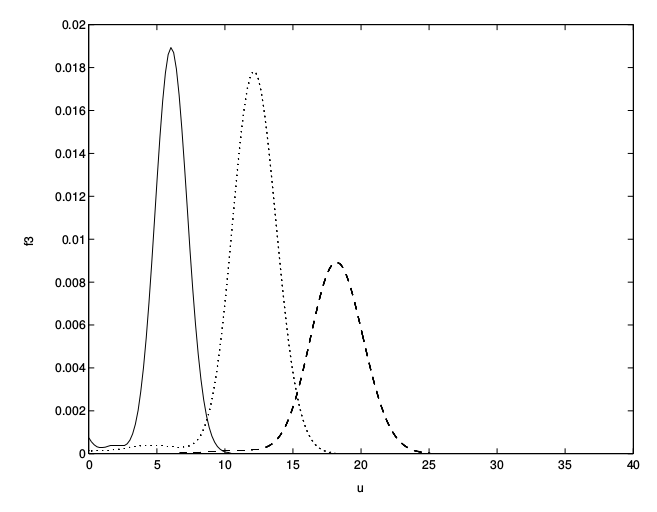
\includegraphics[width=0.8\textwidth]{test2F3.png}
		\caption{Comportamiento de $f_3$, las lineas simbolizan la progresión temporal de $t=2$, $t=8$ y $t=14$ }
		\label{fig:ejemplo3}
	\end{figure}
\end{frame}
\begin{frame}
	\frametitle{Simulaciones numéricas $A_1 = 0.5, A_2 = 0.2, \beta = 1$}
	\begin{figure}
		\centering
		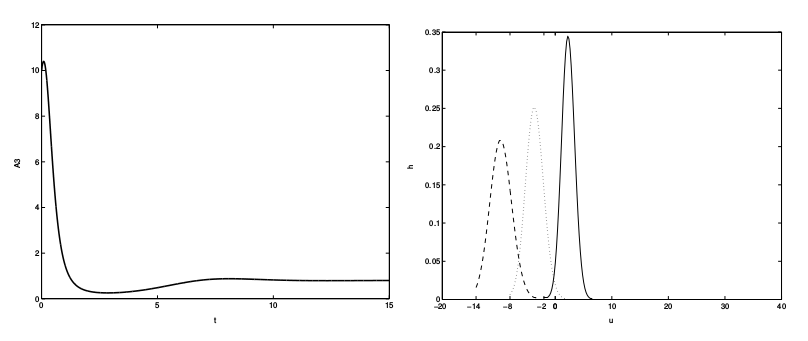
\includegraphics[width=1\textwidth]{test2A3H.png}
		\caption{Comportamiento de $A_3$ y $h$}
		\label{fig:ejemplo4}
	\end{figure}
\end{frame}
\begin{frame}
	\frametitle{Simulaciones numéricas $A_1 = 0.5, A_2 = 0.2, \beta = 10$}
	\begin{figure}
		\centering
		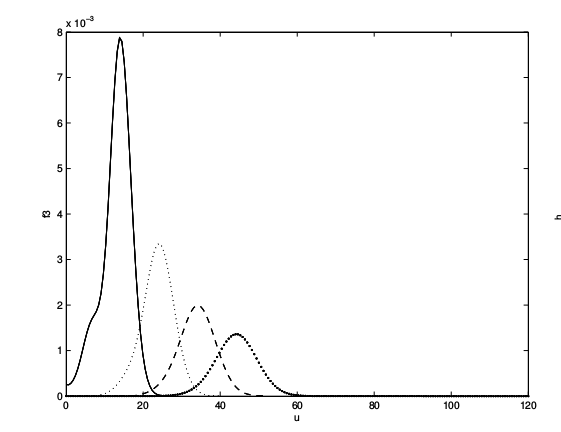
\includegraphics[width=0.8\textwidth]{test222.png}
		\caption{Comportamiento de $f_3$ con $\beta=10$ y condiciones iniciales de caso 2}
		\label{fig:ejemplo5}
	\end{figure}
\end{frame}
\section{Conclusiones y futuro trabajo}

\begin{frame}
  \frametitle{Conclusiones y futuro trabajo}

  \begin{itemize}
    \item Grandes oportunidades biológicas a desarrollar.
    \item Interesantes perspectivas en simulación.
    \item Limitaciones e imprescisiones a subsanar.
  \end{itemize}
\end{frame}

\end{document}
